Here the problem is the same as in the previous step, with the only difference being that also the alpha ratios and the number of products sold for each price are unknown.
Since the learners are not able to distinguish the different types of customers, initially the alphas values (probability to start the interaction from a specific product) are uniformly distributed ($[0.2, 0.2, 0.2, 0.2, 0.2]$) and the number of products bought for each price is set all to 1.\\
The same algorithms as before have been developed, with the additional calculus to estimate the two parameters, now uncertain.

\subsection{UCB-1}
The algorithm repeats the same operations as in the previous chapter from step 1 to step 5. Then, it estimates the two parameters:

\begin{itemize}
    \item estimate alpha ratios $\alpha_{i, t}$:
    \begin{align}
        \sigma_{i, t} = \sigma_{i, t - 1} + starts_{i, t}, \forall i \in \mathcal{P}\\
        \alpha_{i, t} = \frac{\sigma_{i, t}}{\sum_{j \in \mathcal{P}}\sigma_{j, t}},  \forall i \in \mathcal{P}
        \label{eqn:alpha}
    \end{align}Where:\begin{itemize}
        \item $\sigma_{i, t}$ is the number of starts from product $i$ has been observed until time $t$
        \item $starts_{i, t}$ is the number of starting times observed at time $t$ for product $i$
        \item $\mathcal{P}$ is the set of indexes for the products
        \end{itemize}
    \item estimate number of products sold (version 1):\\
    with this first approach, we evaluate these parameters with the empirical mean as can be seen in Equation ~\ref{eqn:num_prod} \begin{equation}
        \label{eqn:mean_items}
        mean\_items[p,a] = \frac{mean\_items[p,a] * seen[p,a] + bought[p]}{estimated\_items[p,a]}
    \end{equation}\begin{equation}
        \label{eqn:num_prod}
        num\_products[p,a] = \frac{1}{mean\_items[p,a]}
    \end{equation}where\begin{itemize}
        \item mean\_items[p,a] is the mean of the number of products {\bf p} with price {\bf a} bought until now
        \item seen[p,a] is the number of times product {\bf p} with price {\bf a} has been bought until the day before
        \item bought[p] is the total amount of products {\bf p} bought on the current day
        \item estimated\_items[p,a] is the number of times products {\bf p} with price {\bf a} have been bought until now (so it is seen[p,a] plus the number of times product p has been bought the current day)
        \item num\_products[p,a] is the inverse of the value computed before because represents the parameter of the Geometric distribution, which we have used to estimate the number of items bought by the customers, once they have decided to buy that product visualized with that price.
    \end{itemize}
    \item estimate number of products sold (version 2):\\
    Since the number of units bought by a customer depends on the price (so, by the chosen arm), we try to use a UCB-1 algorithm to estimate also this parameter. UCB-1 relies on the assumption that the variable we want to estimate has support in $\left[0, 1 \right]$, but the number of units bought belongs to $\left[0, +\infty \right)$, thus we can not directly estimate the number of units with this algorithm.\\
    One possibility is to directly evaluate the parameter of the Geometric distribution (the inverse of the mean). Normally, UCB-1 uses the upper bound to give an optimistic estimate of the parameters in order to induce the exploration of new arms. However, since increasing the parameter of the Geometric distribution will lead to a decrement in the believed estimation of the number of units bought, we will get a pessimistic estimate. To overcome this issue, we subtract the upper bound from the mean, instead of adding.\\
 The results of this version are significantly worse and are not shown below.
\end{itemize}
\subsubsection{Results}
As expected, having less knowledge leads to a solution a little bit worse than the previous step. In other words, the UCB Learner needs more days to converge to the optimal solution. As said before, someday it will change the super arm to pull, in order to explore more.
\begin{figure}[ht]
    \begin{center}
    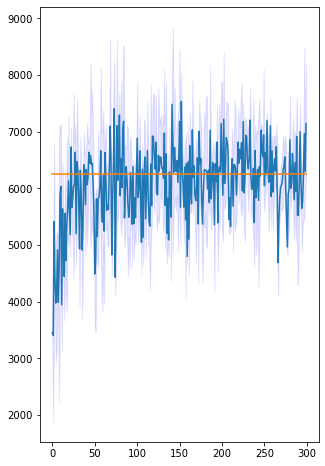
\includegraphics[width=0.6\textwidth]{img/UCB4.png}
    \caption{UCB Reward}
    \label{fig:reward41}
    \end{center}
\end{figure}
\begin{multicols}{2}
    \begin{figure}[H]
        \begin{center}
        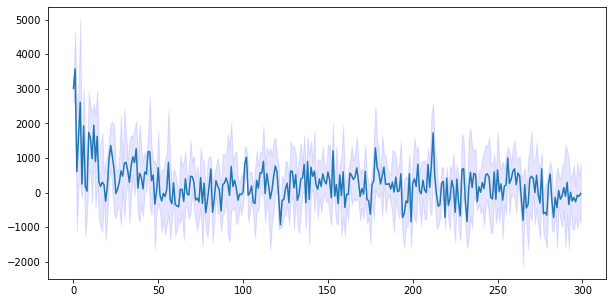
\includegraphics[width=0.5\textwidth]{img/UCB4_regret.png}
        \caption{UCB Regret}
        \label{fig:regret41}
        \end{center}
    \end{figure}
    \columnbreak
    \begin{figure}[H]
        \begin{center}
        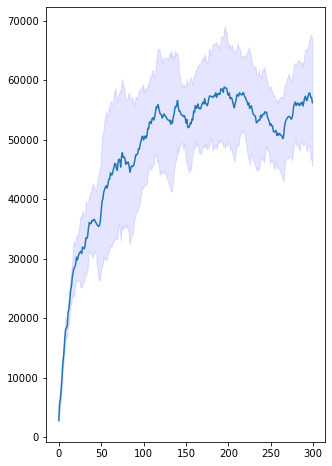
\includegraphics[width=0.5\textwidth]{img/UCB4_cum_reg.png}
        \caption{UCB Cumulative regret}
        \label{fig:cum_reg41}
        \end{center}
    \end{figure}
\end{multicols}

\subsection{TS}
Thomson Sampling estimates the alpha ratios exactly as the UCB with the Equation ~\ref{eqn:alpha}.\\About the estimation of the number of products sold, the method adopted is the same as the second version for the UCB-1. For obvious reasons, the additional parameters are the $\alpha$ and $\beta$ parameters of the Beta distribution used for the additional MAB. The update of $\alpha$ is done as follows:
\begin{align*}
    \alpha[p, a] = \alpha[p, a] + tot\_bought[p]
\end{align*}
where tot\_bought [p] is the total amount of products {\bf p} bought from the first day until now, whereas the update of the $\beta$ parameters is:
\begin{align*}
    \beta[p, a] = \beta [p, a] + seen[p]
\end{align*}
where seen [p] is the number of times the product {\bf p} has been bought until now.\\\\
The two parameters calculated above are updated in the customer's attributes when the learner has to select which super arm to pull.\\

\subsubsection{Results}
The same results as UCB can be observed here, more uncertainty leads to more time to converge. Also this time the results highlight the fact that TS performs better than UCB because it takes less time to converge, generating less cumulative regret.\\ Furthermore, the reason why using the Thompson Sampling algorithm to estimate both the conversion rate and the number of units sold is more effective than UCB-1 might be because it is less explorative. Having two UCB-1 algorithms may lead to too much exploration and less exploitation.
\begin{figure}[ht]
    \begin{center}
    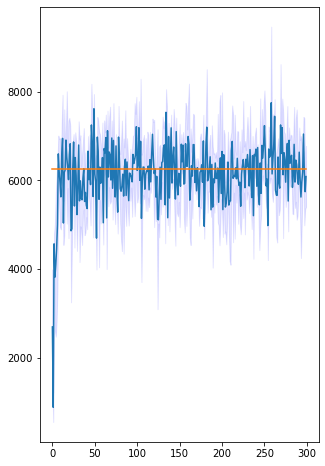
\includegraphics[width=0.6\textwidth]{img/TS4.png}
    \caption{TS Reward}
    \label{fig:reward42}
    \end{center}
\end{figure}
\begin{multicols}{2}
    \begin{figure}[H]
        \begin{center}
        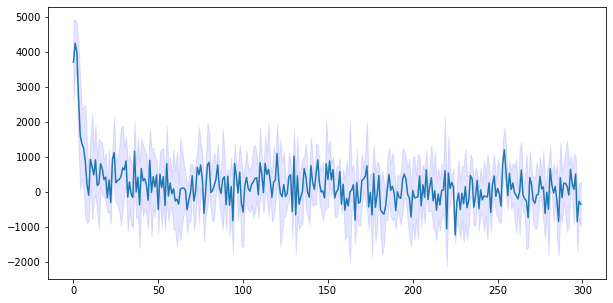
\includegraphics[width=0.5\textwidth]{img/TS4_regret.png}
        \caption{TS Regret}
        \label{fig:regret42}
        \end{center}
    \end{figure}
    \columnbreak
    \begin{figure}[H]
        \begin{center}
        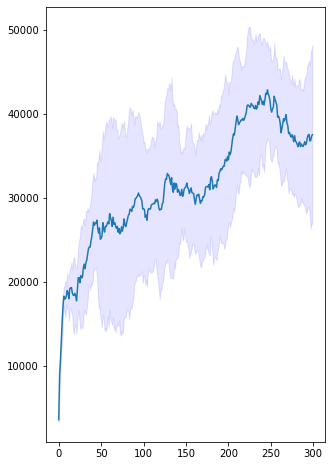
\includegraphics[width=0.5\textwidth]{img/TS4_cum_reg.png}
        \caption{TS Cumulative regret}
        \label{fig:cum_reg42}
        \end{center}
    \end{figure}
\end{multicols}
